Structural assessment of the inflatable configuration has been performed by an estimation of internal forces. This is an essential step in the design of an inflatable aeroshell, since it:
\begin{itemize}
%\item Is required to estimate the inflation pressure to maintain its structural integrity and aerodynamic shape under peak aerodynamic loading
\item Allows to identify whether loads allow for concept structural design within state-of-the-art material capabilities
\item Yields the loads at the structural interface between the inflatable aeroshell and the rigid centre body
\item Gives an impression of the effect of changing design parameters on concept structural performance
\item Gives insight in the structural behaviour and interaction of the inflatable
\end{itemize}
Forces are estimated for an inflatable structure that is aerodynamically loaded, as follows from vehicle trajectory analysis in its deployed condition. An interface with the aerodynamic analysis yields the optimised aeroshell shape as a baseline for the structural model used. 

Moreover, it is essential that mass contributions of centre body, inflatable structure and connections are estimated in order to verify that decelerator mass is below the 1000 [kg] limit imposed as discussed in Chapter \ref{sec:missionreq}. Moreover, the parametric mass model for the inflatable structure allows identification of design venues to minimise structural mass of the decelerator, such that decelerator mass can be minimised and thereby payload mass maximised. 

\subsubsection{Force estimation method}

To meet the purposes of structural assessment of the inflatable configuration, force estimation is performed by a two-dimensional truss analysis on a simplified geometry. This geometry relies on the aerodynamic aeroshell shape as its outer shape. This shape is effected by a number of toroids \gls{sym:N}, held together by radial straps, running along the surface of the inflatable. 

Adjoining toroids are connected at three locations: by a radial strap along the forward side of the aeroshell (impinged by the flow), a radial strap running along the aft side of the aeroshell and at their direct contact surface. In reality, as in the stacked toroid configuration used for NASAs \gls{irve} \cite{Lindell2006}, the contact surface of adjoining toroids is a straight wall, while top and bottom surfaces are of circular shape. This shape is the result of the internally applied pressure: equal but oppositely directed pressures effect a straight interface between toroids and toroids adapt to the unbalanced pressure in top and bottom surfaces through energy minimisation by taking a circular shape.

Simplification was performed to realise a structurally determinate problem results by modelling toroids as diamonds. The orientation of the diamonds is defined by the half-cone angle \gls{sym:theta}, allowed to vary over its radius and circumference per toroid, and their shape by a fixed width \gls{sym:w} and varying height \gls{sym:h}, to allow for a tapered structure. Nodes are designated as the corners of each diamond and connecting members have been numbered. The numbering convention and dimensions are illustrated in Figure \ref{fig:TC}. 

\begin{figure}[ht]
	\centering
	\begin{subfigure}[b]{0.45\textwidth}
	\centering
	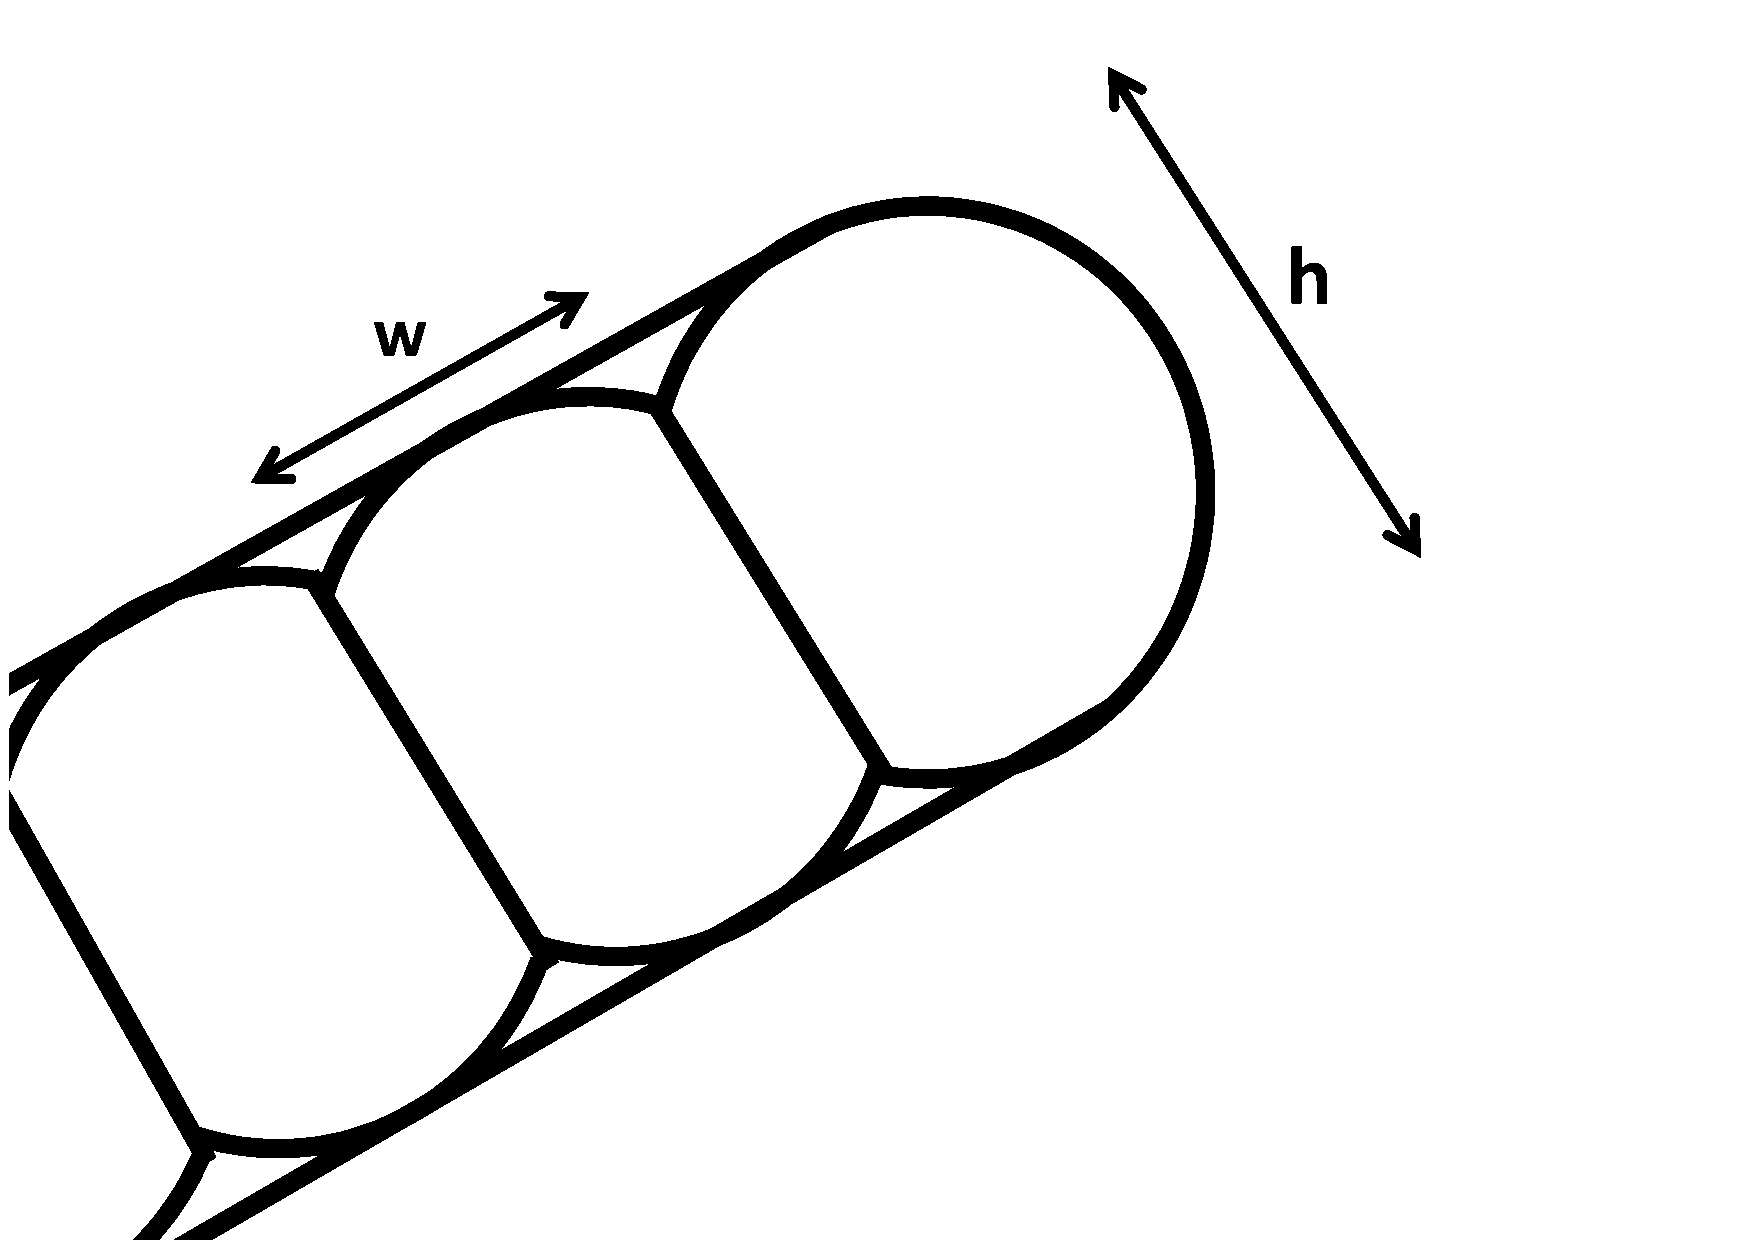
\includegraphics[width=1.0\textwidth]{./Figure/Structure/torconf.pdf}
	\caption{Actual toroid layout} 
	\label{fig:TC1}
	\end{subfigure}
	\begin{subfigure}[b]{0.45\textwidth}
	\centering
	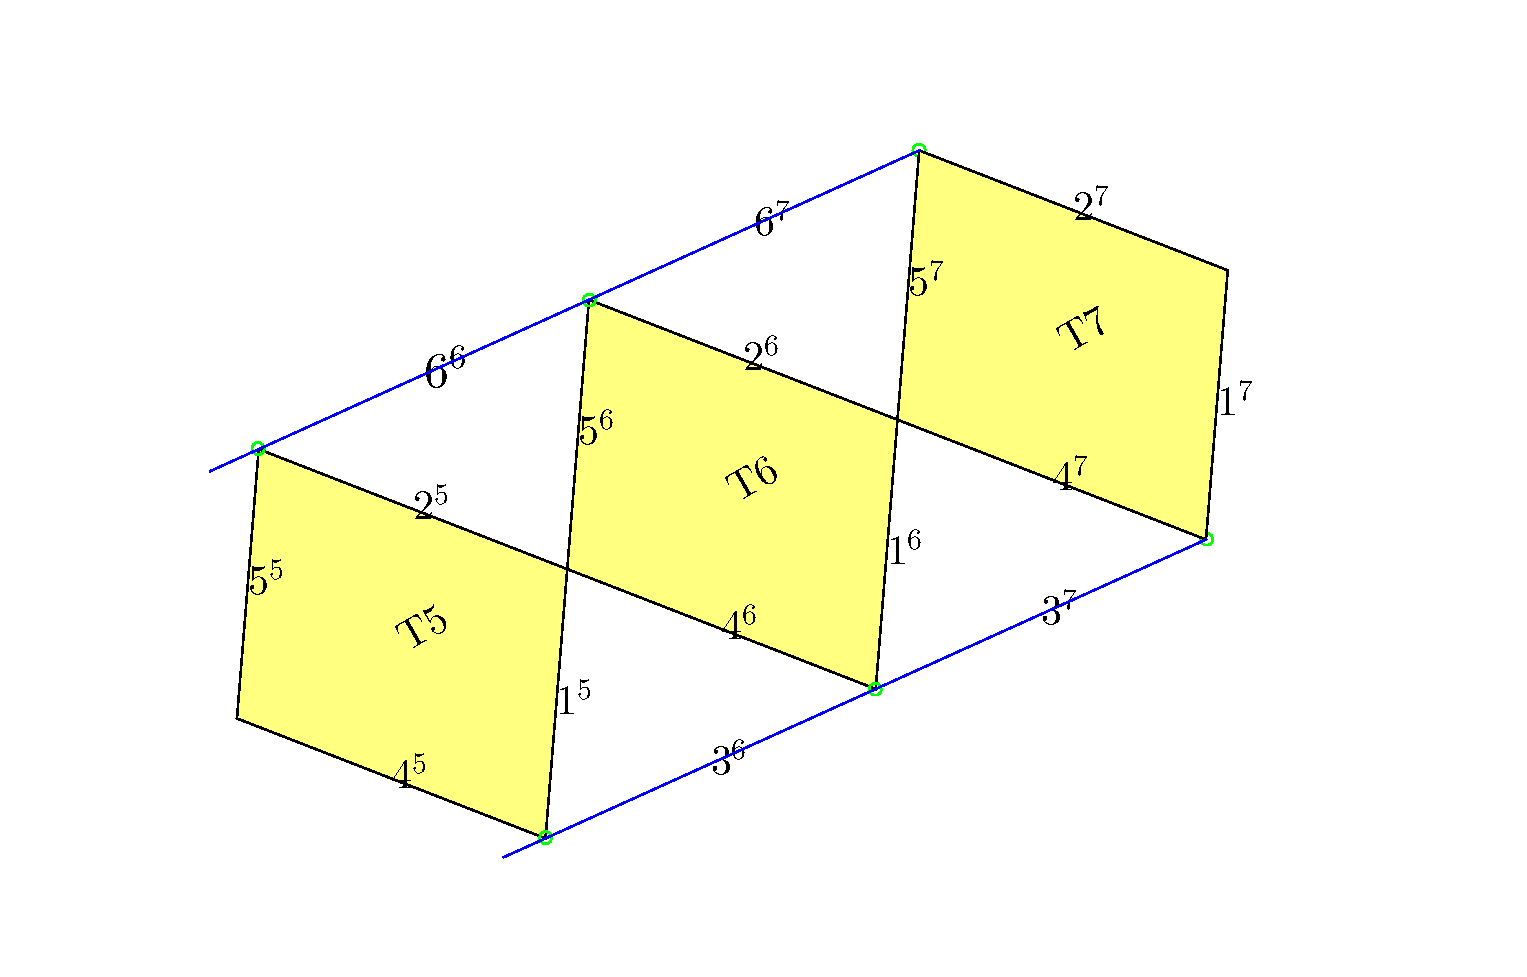
\includegraphics[width=1.0\textwidth]{./Figure/Structure/ToroidConfig2.eps}
	\caption{Simplified truss model} 
	\label{fig:TC2}
	\end{subfigure}
	\caption{Comparison between the actual and simplified inflatable model}
	\label{fig:TC}
\end{figure}

Force estimation is performed in a two-dimensional plane representing a cross-sectional slice, of an infinitesimal angle, of the sphere cone. Each toroid is loaded externally by an aerodynamic force applied perpendicular to its width \gls{sym:w} at its forward node. The aerodynamic force is the resultant of the limit aerodynamic pressure $\gls{sym:q}_{limit}$, assumed constant for each toroid, multiplied by toroid width \gls{sym:w} to represent its working area. 
%The limit aerodynamic pressure is determined from the peak dynamic pressure by multiplying with a \acrfull{fos}, thereby taking into account a contingency for structural design. For composite structures, NASA dictates a \gls{fos} of 1.5 for uniform material and 2.0 for a discontinuity area \cite{Technical2014}. As the inflatable comprises a large amount of component interaction and discontinuity, the ultimate load is calculated as twice the limit aerodynamic pressure that follows from the trajectory analysis in Chapter \ref{ch:XXX}.

%In addition to the aerodynamic pressure acting on the inflatable forward surface, movables (e.g. flaps) at the edge of the aeroshell are taken into account, where present, as a point load directed perpendicular to the flap deployed surface.

As input forces are in Newtons per meter, being the product of a pressure over a length, forces should technically be designated as forces per unit length or running loads. Hereafter, all references to forces in this section are in fact references to running loads. To calculate forces from running loads, these should be multiplied with the circumference over which they act.

On the basis of these external forces, estimation is performed by a truss analysis. By requiring force equilibrium in two orthogonal directions within the plane, internal forces in each of the members 1 to 6 for the \gls{sym:N} toroids are determined. This system of equations is solved from the free end (outboard) to the pinned end (inboard) where the inflatable is connected to the centre body. At this location, reaction forces are determined at the two attachment points, forward and aft.

The decreasing circumference over which forces act going from outboard to inboard in each two-dimensional slice, inherent to the sphere cone design, effects a proportional increase in running loads. This increase is proportional to the decrease in diameter, via the circumference, and thereby member forces are scaled by the ratio of radial distances, with respect to the centre body longitudinal axis, of the nodes they connect.

%Internal pressure is taken into account as follows. It is calculated as the pressure that brings all members into tension, based on the following reasoning. In case members are in compression, buckling will reduce the load-carrying capability of the structure. For the inflatable structure, buckling occurs at low loads due to its flexible and foldable nature. Therefore, the flexible material of the inflatable is not to be loaded into compression and required to be in tension. The latter is effected by the inflation pressure, which is estimated as follows. The first iteration, without inflation pressure, yields internal forces in all members. The requirement for internal pressure is that its induced force $\gls{sym:G}_{infl}$ (or running load), calculated via Equation \ref{eq:pressureforce} \cite{XXX}, brings all members into tension.
%\begin{equation}
%G_{infl} = \frac{p_{infl} w}{2}
%\label{eq:pressureforce}
%\end{equation}
%TDimension \gls{sym:w} is used for all toroids, as it is smaller than \gls{sym:h} and therefore a more conservative estimate for the inflation pressure results. For the outer toroid, the inflation pressure is predominantly carried by the radial straps and this leads to the first requirement that the radial straps are loaded in tension. For all other toroids, the inflation pressure internally balances itself and is thereby not carried through the structure (and radial straps), since cells are symmetric and adjoining cells have the same inflation pressure. This leads to the second requirement that all toroid walls are in tension. Based hereupon, the second iteration proceeds by setting the pressure equal to the value that satisfies the second requirement. Subsequent iterations continue to increase the inflation pressure until the first requirement is met. 
The three-dimensional effects are partially taken into account by assuming that all lateral loads are carried circumferentially rather than in the considered two-dimensional plane. Therefore lateral loads are set to zero at each of the outer (forward and aft) truss nodes. In reality this will, to a large extent, be true as the circular and stacked structure will be the primary contributor to bending stiffness. These lateral loads are primarily those induced by bending moments, such that neglecting them in the two-dimensional plane implies that the bending moment is taken up by the three-dimensional structure. 

The validity of this adjustment is expanded upon in Appendix \ref{sec:VandVstruc} where the verification and validation of the model is discussed. Validation is performed on the basis of \gls{fem} results presented by Lindell et al. \cite{Lindell2006}. The modified two-dimensional method yields acceptable results for force estimations on \gls{irve}-II with a maximum error of 15.4\%, rather than the severe errors induced by not taking into account the three-dimensional bending stiffness. The full verification and validation results can be found in Appendix \ref{sec:VandVstruc}.

The minimum internal pressure required to prevent wrinkling is approximated by Equation \ref{eq:Pmin} \cite{Brown2009, Samareh2011}, based on the premise that the work done by the aerodynamic force $F_{aerodynamic}$ is counteracted by the internal inflation pressure. In this approximation \gls{sym:theta} denotes the mean half-cone angle.
\begin{equation}
\label{eq:Pmin}
\gls{sym:pinfl}_{,min} = F_{aerodynamic} \frac{4}{3 \pi} \frac{tan(\gls{sym:theta})sin(\gls{sym:theta}) }{\gls{sym:Do}\gls{sym:h}}
\end{equation}
This pressure induces a tensile running load $\gls{sym:Q}_{infl}$ in the members of magnitude \cite{Megson2012}
\begin{equation}
\label{eq:Q}
\gls{sym:Q}_{infl} =\frac{\gls{sym:pinfl}_{,min}w}{2}
\end{equation}
Dimension \gls{sym:w} rather than \gls{sym:h} is used as it is the smaller dimension, hence an overestimation of the inflation pressure results. As the pressure calculated by Equation \ref{eq:Pmin} is an approximate minimum inflation pressure for a general stacked toroid case, this value is not necessarily sufficient to bring all members into tension. To this end, inflation pressure is increased to a value that effects tension in all flexible material.

The inputs and outputs of the structural model are tabulated in Table \ref{tab:infl}.
\begin{table}[ht]
\caption{Inflatable structural analysis tool in- and output}
\centering
\begin{tabular}{|l||l|}
\hline
\multicolumn{1}{|c||}{{\bf Input}} & \multicolumn{1}{c|}{{\bf Output}} \\ \hline \hline
Toroid inclination                & Internal forces                   \\ \hline
Number of toroids                 & Reaction forces                   \\ \hline
Toroid dimensions                 & Inflation pressure                \\ \hline
Aerodynamic loading               &                                   \\ \hline
Centerbody and deployed diameter  &                                   \\ \hline
\end{tabular}
\label{tab:infl}
\end{table}

The approach is based on the following assumptions:

\begin{itemize}
\item Small deformations. In reality deformations can be significant changing the orientation and magnitude of forces in the structure.
\item Three-dimensional effects are taken into account by setting the lateral loads to zero. See the previous discussion.
\item Constant dynamic pressure. A constant dynamic pressure is not in line with the actual loading. Based on the discussion in Appendix \ref{sec:VandVstruc}, errors introduced are deemed acceptable.
\item The aerodynamic loading is applied discretely at the outer nodes. The effects of a continuous distribution are neglected since they do not fit within the truss model. This assumptions neglects a bending load within the forward radial strap. 
\item Structural mass is neglected. Neglecting the structural mass causes a small error within the computed loads, varying with the ratio of structural mass and dynamic pressure.
\end{itemize} 
The consequence of these assumptions and their impact, primarily the first two, make the model suitable for a preliminary load analysis of the inflatable structure and the loads at its attachment points, but unsuitable for detailed analysis and structural design and sizing. %To this end, a more detailed model is proposed, namely expanding upon the current model by a \gls{fea}.


%The effects of these assumptions is in total quite significant. The method relies heavily on the first and second assumptions. Considering the foldable nature of the structure, stiffness is limited and actual deformations may become significant. This assumptions is partly taken into account by requiring a inflation pressure which prevents any compressive loading. Still though further stiffness consideration are not taken into account. Based on the significance of these assumptions actual stress distributions can not be considered. However the applied model is reliable for a more general analysis of the structure and the loads.

%The significance of the second assumption is illustrated in Appendix \ref{sec:VandVstruc} discussing the verification and validation of the model. Validation is performed on the basis of \gls{fem} results presented by Lindell et al.. A modified two dimensional method taking into account some of the three dimensional effects yields acceptable results for initial force estimations with a maximum error of 15.4\%. The full verification and validation results can be found in Appendix \ref{sec:VandVstruc}.


\subsubsection{Inflatable mass estimation method}

Mass estimation for the inflatable structure is performed on the basis of a parametric mass model proposed by Samareh \cite{Samareh2011}. The mass model is based on a number of stress equations and cone deformation to compute outputs listed in Table \ref{tab:inflmass}.
\begin{table}[ht]
\caption{Inflatable mass analysis tool in- and output}
\centering
\begin{tabular}{|l||l|}
\hline
\multicolumn{1}{|c||}{{\bf Input}} & \multicolumn{1}{c|}{{\bf Output}} \\ \hline \hline
Toroid inclination         & Flexible material mass            \\ \hline
Centerbody and deployed diameter        & Inflation gas mass                 \\ \hline
Number of toroids                 & Inflation system mass                \\ \hline
Inflation gas properties              &              \\ \hline
Aerodynamic loading               &                                   \\ \hline
Material properties  &                                   \\ \hline
\end{tabular}
\label{tab:inflmass}
\end{table}
Moreover, the model calculates inflation gas pressure based on the premise that work done by inflation gas and aerodynamic pressure should be equal and members are in tension, in line with relations established by Brown \cite{Brown2009}. The model is based on the assumption that the inflatable is an axisymmetric sphere cone of constant half-cone angle, thereby treating a simplified model of the shape determined by aerodynamic optimisation in Section \ref{sec:AeroDesign}. 

Primary assumptions in this model are a symmetric sphere cone and a constant half-cone angle. Verification and validation efforts have been summarised in Appendix \ref{sec:VandVstruc} and have yielded the conclusion that the mass model is suitable for preliminary design.

%Verification has been performed by confirming results reached by Samareh \cite[p.16]{Samareh2011} for nine sample cases, with observed maximum errors of 3 $\%$. Validation has been performed indirectly. The method has been applied in the \gls{edlsa} \cite{Cianciolo2010}, where results showed to be in conformance with high-fidelity \gls{fea} results that have been validated.

%Mass estimation for the centre body structure is performed on the basis of the basic sizing performed in section \label{sec:struc_Centerbody} as the amount of material required to withstand buckling and yielding failure criteria at the ultimate load. Connections are taken into account in the form of a mass margin. [ADD MASS MARGIN] 








